
\setcounter{footnote}{-1}
\SGARefTarget{sga3:ix:chapter:ix}\chapter*{Exposé IX\\
Groups of Multiplicative Type:\\
Homomorphisms into a Group Scheme}
\addcontentsline{toc}{chapter}{Exposé IX. Groups of Multiplicative Type:
Homomorphisms into a Group Scheme}
\markboth{EXPOSÉ IX. GROUPS OF MULTIPLICATIVE TYPE I (HOMOMORPHISMS)}
  {EXPOSÉ IX. GROUPS OF MULTIPLICATIVE TYPE I (HOMOMORPHISMS)}

\begin{center}
  \textit{by A. Grothendieck}\footnote{Editor's note: version 1.0 of
  November 8, 2009. Additions were made in the proof of \SGARefLink{sga3:ix:theorem:3:6:bis}{3.6 bis}, in
  \SGARefLink{sga3:ix:lemma:4:4}{4.4}--\SGARefLink{sga3:ix:theorem:4:7}{7}, \SGARefLink{sga3:ix:lemma:5:0}{5.0}--\SGARefLink{sga3:ix:theorem:5:6}{6}, \SGARefLink{sga3:ix:lemma:6:1}{6.1}, \SGARefLink{sga3:ix:theorem:7:1}{7.1}, and \SGARefLink{sga3:ix:proposition:8:2}{8.2}. Sections \SGARefLink{sga3:ix:proposition:8:1}{8.1} and \SGARefLink{sga3:ix:lemma:4:5}{4.5} remain
  to be revised.}
\end{center}

\SGARefTarget{sga3:ix:section:1}\section*{1. Definitions}
\addcontentsline{toc}{section}{1. Definitions}

\medskip
\noindent\SGARefTarget{sga3:ix:definition:1:1}\textbf{Definition 1.1.} ---
\textit{Let \(S\) be a prescheme and let \(G\) be a group prescheme over
\(S\). The group \(G\) is said to be \emph{of multiplicative type} if it
is locally diagonalizable for the faithfully flat quasi-compact topology
(cf.\ \SGARefLink{sga3:iv:subsection:6:3}{IV 6.3}); that is, if for every \(s\in S\), there are an open
neighborhood \(U\) of \(s\) and a faithfully flat quasi-compact morphism
\(S'\to U\) such that
\[
  G'=G\times_S S'
\]
is a diagonalizable \(S'\)-group (\SGARefLink{sga3:i:subsection:4-4}{I 4.4} and \SGARefLink{sga3:viii:definition:1:1}{VIII 1.1}).}

\textit{The group \(G\) is said to be \emph{of quasi-isotrivial
multiplicative type} if it is locally diagonalizable even for the étale
topology (\SGARefLink{sga3:iv:subsection:6:3}{IV 6.3}); that is, if in the preceding definition one can take
\(S'\to U\) to be étale and surjective. Equivalently---as one sees by
taking the disjoint union of the schemes \(S'\) attached to the various
\(s\in S\)---there is an étale surjective morphism \(S'\to S\) such that
\(G'=G\times_S S'\) is a locally diagonalizable \(S'\)-group.}

\textit{If one can moreover choose \(S'\to S\) to be finite, étale, and
surjective, then \(G\) is said to be \emph{of isotrivial multiplicative
type}.}

\textit{Finally, \(G\) is said to be a group \emph{of locally trivial
multiplicative type} (respectively, \emph{of locally isotrivial
multiplicative type}) if every \(s\in S\) has an open neighborhood \(U\)
such that \(G\times_S U\) is a diagonalizable \(U\)-group (respectively,
is of isotrivial multiplicative type; in other words, there is a finite
étale surjective morphism \(S'\to U\) such that \(G\times_S S'\) is a
diagonalizable \(S'\)-group).}

\medskip
\noindent\SGARefTarget{sga3:ix:comments:1:2}\textbf{Comments 1.2.} ---
The five preceding notions are all obtained from the notion of a
diagonalizable group by localization, with respect to five different
``topologies'' associated with \((\mathbf{Sch})\).

It is understood in general that, when the word ``locally'' is not
qualified by naming the topology under consideration, the Zariski
topology is meant, in accordance with established terminology. In the
terminology introduced here, ``of locally trivial multiplicative type''
is equivalent to ``locally diagonalizable'' in \SGARefLink{sga3:viii:definition:1:1}{VIII 1.1}; likewise,
``trivial'' translates as ``diagonalizable.'' The five notions introduced
above fit into the following implication diagram, which follows from the
corresponding relations among the topologies involved:

\SGARefTarget{sga3:ix:diagram:1:2}
\begin{center}
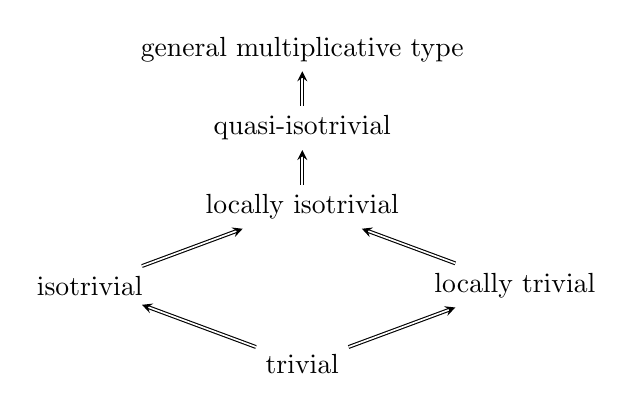
\begin{tikzpicture}[>=stealth]
  \node (general) at (0,4.0) {general multiplicative type};
  \node (quasi) at (0,3.0) {quasi-isotrivial};
  \node (lociso) at (0,2.0) {locally isotrivial};
  \node (iso) at (-2.7,1.0) {isotrivial};
  \node (loctriv) at (2.7,1.0) {locally trivial};
  \node (triv) at (0,0) {trivial};
  \draw[double,->] (quasi) -- (general);
  \draw[double,->] (lociso) -- (quasi);
  \draw[double,->] (iso) -- (lociso);
  \draw[double,->] (loctriv) -- (lociso);
  \draw[double,->] (triv) -- (iso);
  \draw[double,->] (triv) -- (loctriv);
\end{tikzpicture}
\end{center}

For practical purposes, let us point out at once that every group of
multiplicative type that we shall encounter will be quasi-isotrivial. Thus
we shall see in the next exposé (\SGARefLink{sga3:x:corollary:4-5}{X 4.5}) that, when \(G\) is of finite type
over \(S\), it is automatically quasi-isotrivial; we shall nevertheless
give examples in which it is not locally isotrivial. We shall likewise see
that \(G\) may be locally trivial without being isotrivial, and hence
\emph{a fortiori} without being trivial. This readily implies that the
inclusions in \SGARefLink{sga3:ix:diagram:1:2}{the preceding diagram} are strict.

On the other hand, we shall also see there (\SGARefLink{sga3:x:theorem:5-16}{X 5.16}) that, when \(S\) is
locally noetherian and normal---or, more generally, geometrically
unibranch---every group of multiplicative type and finite type over \(S\)
is necessarily isotrivial; moreover, it is trivial as soon as it is
locally trivial (or even merely trivial over a dense open subset). This
explains why most groups of multiplicative type encountered in practice
will doubtless be isotrivial, all the more so because we shall later see
that the maximal tori of semisimple group schemes are automatically
isotrivial.

\medskip
\noindent\SGARefTarget{sga3:ix:definition:1:3}\textbf{Definition 1.3.} ---
\textit{Let \(S\) and \(G\) be as in
\SGARefLink{sga3:ix:definition:1:1}{1.1}. The group \(G\) is called a
\emph{torus} if, for the faithfully flat quasi-compact topology, it is
locally isomorphic to a group of the form \(\mathbf G_m^r\), where
\(r\) is an integer with \(r\geq 0\).}

With the notation of \SGARefLink{sga3:ix:definition:1:1}{1.1}, this says
that \(S'\) may be chosen so that \(G'\) is isomorphic to a group of the
form \((\mathbf G_{m,S'})^r\). The integer \(r\) depends on \(s\in S\):
it is the dimension of the fiber
\[
  G_s=G\otimes_S\kappa(s).
\]
It is a locally constant function of \(s\), as is seen at once. This
observation should be generalized as follows.

\medskip
\noindent\SGARefTarget{sga3:ix:definition:1:4}\textbf{Definition 1.4.} ---
\textit{Let \(G\) be a diagonalizable group scheme over a field \(k\).
Thus \(G\) is isomorphic to a group \(D_k(M)\), where \(M\) is an ordinary
commutative group determined up to isomorphism by this condition---more
precisely,
\[
  M\simeq\operatorname{Hom}_{k\text{-}\mathrm{gr}}
    (G,\mathbf G_{m,k})
\]
(\SGARefLink{sga3:viii:corollary:1:3}{VIII 1.3}). The isomorphism class of \(M\) is called the \emph{type} of
the diagonalizable group \(G\); it is plainly invariant under extension
of the base field.}

\textit{Now let \(G\) be a group scheme of multiplicative type over an
arbitrary prescheme \(S\). For every \(s\in S\), there is an extension
\(k\) of \(\kappa(s)\) such that
\(G\times_S\operatorname{Spec}(k)\) is a diagonalizable
\(k\)-group.\footnote{Editor's note: indeed, by hypothesis there are an
open neighborhood \(U\) of \(s\) and a faithfully flat quasi-compact
morphism \(S'\to U\) such that \(G_{S'}\) is diagonalizable. For every
\(s'\in S'\) above \(s\), the field \(\kappa(s')\) is an extension of
\(\kappa(s)\), and
\(G_{s'}=G\times_S\operatorname{Spec}(\kappa(s'))\) is diagonalizable.}
Its type is independent of the chosen extension by the preceding
observation and is called the \emph{type of \(G\) at \(s\)}, or the
\emph{type of \(G_s\)}. In particular, if \(G\) itself is diagonalizable,
and hence isomorphic to a group of the form \(D_S(M)\), then for every
\(s\in S\) the type of \(G\) at \(s\) is the isomorphism class of \(M\).}

\textit{More generally, if \(G\) is a group of multiplicative type over
\(S\) and \(M\) is an ordinary commutative group, then \(G\) is said to
be \emph{of type \(M\)} if it is of type \(M\) at every point \(s\in S\);
equivalently, if \(G\) is locally isomorphic to \(D_S(M)\) for the
faithfully flat quasi-compact topology.}

\medskip
\noindent\SGARefTarget{sga3:ix:remark:1:4:1}\textbf{Remark 1.4.1.}
\footnote{Editor's note: the number \SGARefLink{sga3:ix:remark:1:4:1}{1.4.1} has been added to the remarks
that follow, for use in later references.}
\SGARefTarget{sga3:ix:remark:1:4:1:item:a}\textit{a) For a group \(G\) of multiplicative type over \(S\), the
function
\[
  s\longmapsto \text{the type of }G_s
\]
is locally constant on \(S\). Indeed, with the notation of
\SGARefLink{sga3:ix:definition:1:1}{1.1}, if \(G'\) is of type \(M\),
then \(G\) is of type \(M\) over the neighborhood \(U\) of \(s\).
Consequently \(S\) has a canonical decomposition as a disjoint union of
preschemes \(S_i\) such that, for every \(i\), \(G_{S_i}\) is of type
\(M_i\), where the commutative groups \(M_i\) are pairwise
nonisomorphic.}

\SGARefTarget{sga3:ix:remark:1:4:1:item:b}\textit{b) In particular, if \(S\) is connected, the type of the fibers
of \(G\) is constant; that is, there is a commutative group \(M\) such
that \(G\) is of type \(M\). Finally, if \(G\) is a torus, the type of
\(G\) at \(s\) is determined by the integer \(\dim G_s\): indeed,
\(G_s\) is of type \(\mathbb Z^n\), where \(n=\dim G_s\).}

\medskip
\noindent\SGARefTarget{sga3:ix:remark:1:5}\textbf{Remark 1.5.} ---
\SGARefTarget{sga3:ix:remark:1:5:item:a}\textit{a) It follows immediately from Definitions
\SGARefLink{sga3:ix:definition:1:1}{1.1} and
\SGARefLink{sga3:ix:definition:1:3}{1.3} that these notions are
``compatible with base extension.'' Thus, if \(G\) is a group prescheme
over \(S\) and \(S'\to S\) is a base-change morphism, then whenever \(G\)
is of multiplicative type (respectively, of isotrivial multiplicative
type, and so on), the same is true of \(G'\).}

\SGARefTarget{sga3:ix:remark:1:5:item:b}\textit{b) If, moreover, \(S'\to S\) is faithfully flat and
quasi-compact, then \(G'\) being of multiplicative type, respectively a
torus, implies the same for \(G\). If \(S'\to S\) is also étale
(respectively, finite étale), then \(G'\) being quasi-isotrivial
(respectively, isotrivial) implies the same for \(G\).}

\SGARefTarget{sga3:ix:remark:1:5:item:c}\textit{c) Finally, return to an arbitrary base-change morphism
\(f:S'\to S\). If \(s'\in S'\) and \(s=f(s')\), then the type of \(G'\)
at \(s'\) is the same as that of \(G\) at \(s\), since
\[
  G'_{s'}=G_s\otimes_{\kappa(s)}\kappa(s').
\]}
